\textbf{\LARGE dop 31. Закон Амдала, его следствия. Этапы решения задач на параллельных вычислительных системах. Граф алгоритма, критический путь графа алгоритм, ярусно-параллельная форма графа алгоритма.}\\

\begin{itemize}
    \item $p$ – число процессоров (ядер, вычислительных узлов)
    \item $T_{1}$ – время работы программы на одном процессоре
    \item $T_{p}$ – время работы программы на системе из $p$ процессоров
    \item $S = \frac{T_{1}}{T_{p}}$ – это ускорение работы программы при переходе с одного процессора на систему из $p$ процессоров (во сколько раз
программа начинает работать быстрее)
    \item $f$ – доля последовательных операций в исходной программе ($0 \leq f \leq 1$).
\end{itemize}

\textbf{Закон Амдала}\\
Ускорение работы программы при переходе с одного процессора на систему из $p$ процессоров можно оценить следующим образом:
\begin{center}
$S \leq \frac{1}{f + \frac{1 - f}{p}}$
\end{center}

\textbf{Следствия}:\\
1) $S \approx \frac{1}{f}$ (при большом числе процессоров)\\
На практике. Если доля последовательных операций в некоторой программе равна 0.1, значит вне зависимости от числа используемых процессоров ускорение не превысит 10.\\

2) В теории. Для того чтобы ускорить программу в $q$ раз, необходимо ускорить не менее, чем в $q$ раз не менее, чем $(1-\frac{1}{q})$-ю часть программы.
На практике. Нужно ускорить работу программы в 100 раз. Значит необходимо ускорить не менее, чем в 100 раз не менее, чем 99\% этой программы.\\

\textbf{Граф управления.} Каждому оператору исходной программы ставится соответствие вершина графа, дугами в этом графе выступают переходы в состояния, описанные вершинами графа.\\

\textbf{Информационный граф.} Среди операторов принимаются во внимание только преобразователи, а в качестве отношения между ними брать отношение информационной зависимости. Сначала строится граф, в котором вершины соответствуют операторы-преобразователи. Две вершины соединяются информационной дугой, если между ними какими-нибудь срабатываниями соответствующих операторов теоретически возможна информационная связь. Информационный граф не зависит от входных данных. Информационная зависимость определяет критерий эквивалентности преобразований программ.
Информационная независимость определяет ресурс параллелизма программы.\\

\textbf{Ярусно-параллельная форма графа алгоритма.}
Начальная вершина каждой дуги расположена на ярусе с номером меньшим, чем номер яруса конечной вершины. Между вершинами, расположенными на одном ярусе, не может быть дуг.\\
\begin{itemize}
    \item Высота ЯПФ – это число ярусов.
    \item Ширина яруса – число вершин, расположенных на ярусе.
    \item Ширина ЯПФ – это максимальная ширина ярусов в ЯПФ.
    \item Высота ярусно-параллельной формы - это сложность параллельной реализации алгоритма или программы.
\end{itemize}

Ярусно-параллельная форма называется \textbf{канонической}, если у любой вершины, кроме вершин первого яруса, есть входная дуга, идущая с предыдущего яруса.\\
Высота канонической ЯПФ = длине критического пути + 1. Критический путь в ориентированном ациклическом графе – это путь максимальной длины.
\begin{center}
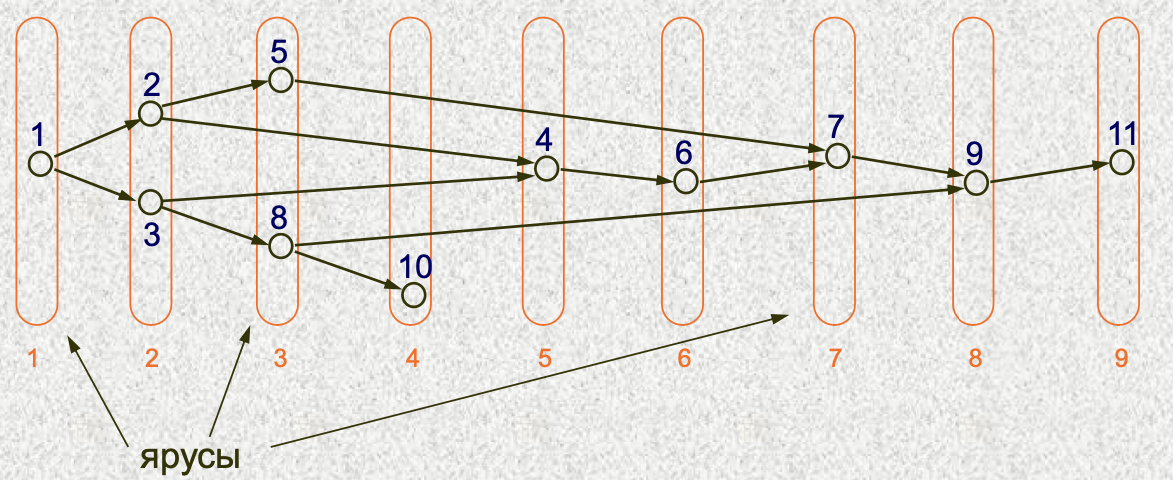
\includegraphics[width=0.6\textwidth]{pics/layered-graph-algo.png}
\end{center}

% -------- source --------
\bigbreak
[\cite{super_computers_lections} 134-137, 709-714]